\begin{tikzpicture}
	\node[namedVertex] (s) at (0,0) {$s$};
	\node[namedVertex] (v) at (4,0) {$v$};
	\node[namedVertex] (w) at (8,0) {$w$};
	\node[namedVertex] (t)  at (12,0) {$t$};
	
	\draw[edge] (s) -- node[below](e0){$e_0$} node[above]{$\tau_{e_0}=1, \nu_{e_0}=4$} (v);
	\draw[edge] (v) to[bend left=30] node[below]{$e_1$} node[above]{$\tau_{e_1}=2, \nu_{e_1}=2$} (w);
	\draw[edge] (v) to[bend right=30] node[above]{$e_2$} node[below]{$\tau_{e_2}=2, \nu_{e_2}=2$} (w);
	\draw[edge] (w) -- node[below]{$e_3$} node[above](e3){$\tau_{e_3}=2, \nu_{e_3}=\infty$} (t);
	
	\node[above of=e3, anchor=south,node distance=.3cm] {
		\begin{tikzpicture}[scale=1,solid,black,
			declare function={
				c(\x)= 2;			
			}]
			
			
			\begin{axis}[xmin=0,xmax=6.5,ymax=4.5, ymin=0, samples=500,width=5.5cm,height=3cm,
				axis x line*=bottom, axis y line*=left, axis lines=middle, xtick={1,2,3,4,5,6}, ytick={2,4}]
				\addplot[blue, ultra thick,domain=0:7] {c(x)} node[above,pos=.5]{$c_{e_3}$};
			\end{axis}
			
		\end{tikzpicture}
	};

	\node[above of=e0, anchor=south,node distance=.8cm] {
		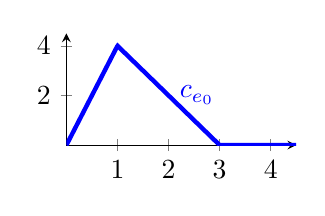
\begin{tikzpicture}[scale=1,solid,black,
			declare function={
				c(\x)= and(\x >= 0, \x <= 1)*4*\x + and(\x > 1, \x <=3)*(6-2*\x);			
			}]
			
			
			\begin{axis}[xmin=0,xmax=4.5,ymax=4.5, ymin=0, samples=500,width=4.5cm,height=3cm,
				axis x line*=bottom, axis y line*=left, axis lines=middle, xtick={1,2,3,4}]
				\addplot[blue, ultra thick,domain=0:5] {c(x)} node[right,pos=.6]{$c_{e_0}$};
			\end{axis}
			
		\end{tikzpicture}
	};	

	\node[left of=s,blue](){$Q=4$};
\end{tikzpicture}
